%%%%%%%%%%%%%%%%%%%%%%%%%%%%%%%%%%%%%%%%%%%%%%%%%%%%%%%%%%%%%%%%%%%%%%%%%%%%
%% main.tex -- Signal-peptide prediction report (OUP authoring template)
%%
%% Compile on Overleaf with the oup-authoring-template.cls in the project.
%% Figures are read from the repository's data/ directory; if you compile
%% outside the repo, copy the referenced PDFs next to this file or fix paths.
%%
%% All tables/numbers reflect the regenerated pipeline (seeded split, fixed
%% von Heijne fold selection). The feed-forward neural network is included.
%%%%%%%%%%%%%%%%%%%%%%%%%%%%%%%%%%%%%%%%%%%%%%%%%%%%%%%%%%%%%%%%%%%%%%%%%%%%

\documentclass[unnumsec,webpdf,contemporary,large]{oup-authoring-template}

\usepackage{booktabs}
\usepackage{graphicx}
\usepackage{amsmath}

\begin{document}

\journaltitle{Laboratory of Bioinformatics}
\DOI{}
\copyrightyear{2026}
\pubyear{2026}
\access{}
\appnotes{Project Report}

\firstpage{1}

\title[von Heijne, SVM and FFNN Models for Signal Peptide Prediction]{Comparison of von Heijne, Support Vector Machine and Feed-Forward Neural Network Models for Signal Peptide Prediction}

\author[1]{Nikita Leino}
\author[2]{Vanessa El Debs}

\authormark{Leino and El Debs}

\address[1]{\orgdiv{FABIT}, \orgname{University of Bologna}, \orgaddress{\postcode{40131}, \city{Bologna}, \country{Italy}}, \email{nikita.leino@studio.unibo.it}}
\address[2]{\orgdiv{FABIT}, \orgname{University of Bologna}, \orgaddress{\postcode{40131}, \city{Bologna}, \country{Italy}}, \email{vanessa.eldebs@studio.unibo.it}}

\abstract{Signal peptides mediate protein translocation within the eukaryotic secretory pathway. Given the high costs associated with experimental validation, robust \textit{in silico} prediction tools are of critical importance for applications ranging from genome annotation to disease diagnosis. This work compares the efficacy of a von Heijne-based statistical method against two machine-learning approaches---a Support Vector Machine (SVM) and a feed-forward neural network (FFNN)---for signal peptide classification. Although the von Heijne method performs reliably on canonical motifs, it struggles with non-canonical sequence compositions and confuses N-terminal transmembrane helices with signal-peptide hydrophobic cores. In contrast, the feature-based machine-learning models, trained on the same physicochemical features, achieved markedly higher overall accuracy and Matthews Correlation Coefficient (MCC), proving to be more effective tools for signal peptide prediction.}

\keywords{SP, SVM, FFNN, ML, von Heijne}

\maketitle


\section{Introduction}

Intracellular protein distribution is a strictly regulated process, as the functional efficacy of a protein is contingent upon its delivery to the specific subcellular compartment that provides the requisite biochemical environment \cite{ref1}. Numerous protein-sorting processes used by eukaryotic cells are mediated by N-terminal targeting signals \cite{ref1}. Disruptions in these trafficking pathways or subsequent protein mislocalization are implicated in a broad spectrum of human pathologies \cite{ref5}.

Protein translocation into the eukaryotic secretory system or across prokaryotic membranes is coordinated by signal peptides (SPs), which are N-terminal sequences that are usually 15--30 residues long \cite{ref17,ref20}. As illustrated in Figure~\ref{fig:sp}, SPs possess a characteristic tripartite architecture:

\begin{enumerate}
\item \textbf{The N-region:} An amino-terminal segment enriched with positively charged residues, such as lysine, arginine, and histidine.
\item \textbf{The H-region:} A central hydrophobic core, which frequently adopts an $\alpha$-helix conformation.
\item \textbf{The C-region:} A polar/neutral carboxyl-terminal segment containing a weakly conserved cleavage site that facilitates precise proteolytic processing following translocation \cite{ref23}.
\end{enumerate}

SPs are essential to many biotechnological and medicinal applications, such as genome annotation, recombinant protein expression, diagnostic discovery, and vaccine creation, because of these structural characteristics \cite{ref17,ref20,ref23}.

Accurately identifying SPs is essential to predicting subcellular localization because they are the major factors for protein entrance into the secretory pathway. Nevertheless, experimental validation of SPs continues to be time-consuming, labor-intensive, and frequently vulnerable to cell-type or condition-specific variability \cite{ref23,ref6}. These constraints have catalyzed the development of \textit{in silico} prediction tools, which provide scalable, rapid, and reproducible alternatives \cite{ref13}. Computational inference of subcellular localization is now crucial for the functional annotation of uncharacterized proteomes by bridging the gap between raw sequence data and biological knowledge \cite{ref8}.

The methodological landscape for SP prediction has evolved significantly over several decades \cite{ref16}. Early weight-matrix models \cite{ref22} laid the groundwork for more sophisticated feature-based classifiers, such as Support Vector Machines (SVMs) \cite{ref21,ref7} and Random Forests \cite{ref14}. Subsequent advancements introduced probabilistic and homology-based frameworks, including Hidden Markov Models \cite{ref4}, eventually culminating in modern deep-learning architectures \cite{ref20,ref18}. These deep-learning approaches currently define the state-of-the-art, as they can autonomously extract complex, non-linear sequence patterns from raw data and demonstrate superior generalization across diverse species and SP classes \cite{ref20,ref18,ref2,ref12}.

The aim of this project is to evaluate the comparative efficacy of distinct computational paradigms for SP detection: von Heijne's (vH) positional scoring matrices and feature-based machine-learning strategies (an SVM and a feed-forward neural network). By benchmarking these methods against a common curated dataset, we assessed their capacity to capture the fundamental physicochemical properties of SPs and their ability to generalize to novel sequences. Our results indicate that while the vH method remains effective for identifying canonical motifs, the machine-learning approaches achieve higher overall accuracy and MCC by integrating diverse, sequence-derived features. Furthermore, our benchmarking highlights the characteristic false-positive and false-negative profiles inherent to each methodology, providing insights into their respective predictive limitations.

\begin{figure}[t]
\centering
% Replace with your original schematic if available.
% \includegraphics[width=\linewidth]{figures/sp_schematic.pdf}
\caption{Schematic representation of a canonical SP. The SP contains an N-terminal region (1--5 residues), an H-region (7--15 residues), and a C-region (3--7 residues).}
\label{fig:sp}
\end{figure}


\section{Materials and Methods}

\subsection{Computational Environment and Software Stack}

The \textit{Python 3} programming environment was used to create the computational framework for this investigation, which adopted a modular architecture intended for repeatable bioinformatics analysis. The \textit{Pandas} and \textit{NumPy} libraries were used for data processing and structural manipulation of the main \textit{UniProtKB} datasets. This allowed for effective numerical operations and the creation of high-dimensional feature vectors. To ensure environment stability and cross-platform reproducibility, the \textit{Conda} package manager was utilized for dependency management and environment isolation.

The machine learning workflow was primarily managed via the \textit{Scikit-learn} library. This included the entire pipeline from data preprocessing---specifically feature normalization using the \textit{StandardScaler}---to the implementation of the Support Vector Machine (SVM) classifier (the \textit{SVC} module) and the feed-forward neural network (the \textit{MLPClassifier} module). Model performance was quantitatively assessed through validated metric implementations (Accuracy, MCC, precision, recall and F1), and classification efficacy was qualitatively evaluated through Precision--Recall (PR) curves. For comparative benchmarking, a baseline was established using an implementation of the von Heijne (vH) algorithm \cite{ref22}, developed using \textit{NumPy} for vectorized scoring-matrix calculations. Statistical visualization was executed using the \textit{Matplotlib} and \textit{Seaborn} libraries.

\subsection{Data Collection and Preprocessing}

The \textit{UniProtKB} database provided high-quality sequence data for both signal peptide-positive (SP+) and signal peptide-negative (SP--) cases. A bespoke Python script created for reliable query management and data cleansing was used to automate data retrieval using the UniProt REST API. Several rigorous filters were used to create a high-confidence dataset of eukaryotic proteins with experimentally verified SPs. The first query required ``Evidence at the protein level,'' was limited to ``Reviewed'' (Swiss-Prot) entries, and was restricted to the \textit{Eukaryota} superkingdom. Additionally, fragments and sequences shorter than 40 residues were excluded; only sequences with an empirically verified SP were retained. As UniProtKB does not support direct filtering by SP length, an additional custom filter was implemented to retain only proteins possessing an SP of $\geq 14$ residues. This process yielded 2{,}960 positive entries.

The negative dataset was designed to represent non-secretory proteins with definitive subcellular localizations. The same quality filters (Eukaryota, reviewed, protein-level evidence, and minimum length) were applied. Critically, an exclusion filter was used to remove any protein with any reported evidence of an SP. To ensure a strictly non-secretory identity, proteins were required to have experimental evidence for localization in one of the following compartments: cytosol, nucleus, mitochondrion, plastid, peroxisome, or cell membrane. This query yielded 20{,}944 negative entries.

To mitigate biases arising from over-represented protein families or organisms, both datasets were subjected to a redundancy-reduction pipeline. Sequences were clustered using MMseqs2 \cite{ref19} with a minimum sequence identity threshold of 30\%, an alignment coverage of 40\%, and the connected-component clustering mode. Selecting one representative sequence per cluster ensures a higher level of model generalization, leaving 1{,}103 non-redundant positive and 9{,}076 non-redundant negative sequences.

Crucially, redundancy reduction was performed on the \emph{complete} positive and negative sets \emph{before} any partitioning, so that no homologous pair can be split between training and benchmarking data. In order to preserve the initial positive-to-negative ratio, the non-redundant sequences were then shuffled with a fixed random seed and randomly divided into a training set (80\%) and a benchmarking set (20\%). The training data were further divided into five folds for cross-validation, with fold assignments recorded in the metadata to ensure reproducibility and prevent data leakage. Associated metadata, including UniProt accession, taxonomic lineage, SP cleavage-site position, and the presence of transmembrane (TM) domains within the N-terminal 90 residues, were exported to a TSV file. For SP-- sequences, the cleavage site was set to 0. For the TM feature, positive sequences were labeled ``NIL,'' while negative sequences were assigned a Boolean flag. The final dataset statistics are summarized in Table~\ref{tab:composition}.

\begin{table}[t]
\caption{Composition of the benchmarking set and cross-validation training folds (non-redundant sequences).}
\label{tab:composition}
\centering
\begin{tabular}{lrrr}
\toprule
Dataset Split & Negative & Positive & Total \\
\midrule
Benchmarking & 1816 & 221 & 2037 \\
Fold 1 & 1452 & 176 & 1628 \\
Fold 2 & 1452 & 176 & 1628 \\
Fold 3 & 1452 & 177 & 1629 \\
Fold 4 & 1452 & 176 & 1628 \\
Fold 5 & 1452 & 177 & 1629 \\
\midrule
Total & 9076 & 1103 & 10179 \\
\bottomrule
\end{tabular}
\end{table}

A descriptive analysis was conducted to characterise the training and benchmarking subsets. The dataset is imbalanced, with roughly 7.1 negatives per positive, and the two classes differ taxonomically: positives are dominated by \textit{Metazoa} (82.6\%), whereas negatives are more evenly spread across \textit{Metazoa} (60.2\%), \textit{Viridiplantae} (19.7\%) and \textit{Fungi} (18.2\%). At the species level, \textit{Homo sapiens} alone provides 25\% of the positives and 30\% of the negatives, with the negative set further concentrated in a few model organisms (mouse, \textit{Arabidopsis}, \textit{S.\ cerevisiae}). This taxonomic skew is relevant for interpretation: the model is trained predominantly on animal signal peptides, so its behaviour on plant and fungal SPs is effectively extrapolation and the reported metrics may not transfer uniformly across kingdoms (Figure~\ref{fig:kingdom}). Positive sequences are also markedly shorter than negatives (median 214 vs.\ 436 residues; Figures~\ref{fig:lendist}--\ref{fig:lenout}), although only the first 40--90 residues enter the features, so this length difference does not directly bias the classifiers.

In accordance with standard signal-peptide profiles, SP lengths among SP+ sequences varied from roughly 14 to 60 amino acids, peaking at 20--25 residues (median 22; Figure~\ref{fig:splen}). A high over-representation of apolar residues, especially leucine and alanine, together with a depletion of charged residues relative to the \textit{UniProtKB/Swiss-Prot} baseline \cite{ref3}, was revealed by residue-composition analysis. Sequence-logo analysis \cite{ref11} for the region spanning 13 positions upstream to 2 positions downstream of the cleavage site confirmed the presence of the hydrophobic core and the conserved A-X-A motif across both subsets.

\begin{figure}[t]
\centering
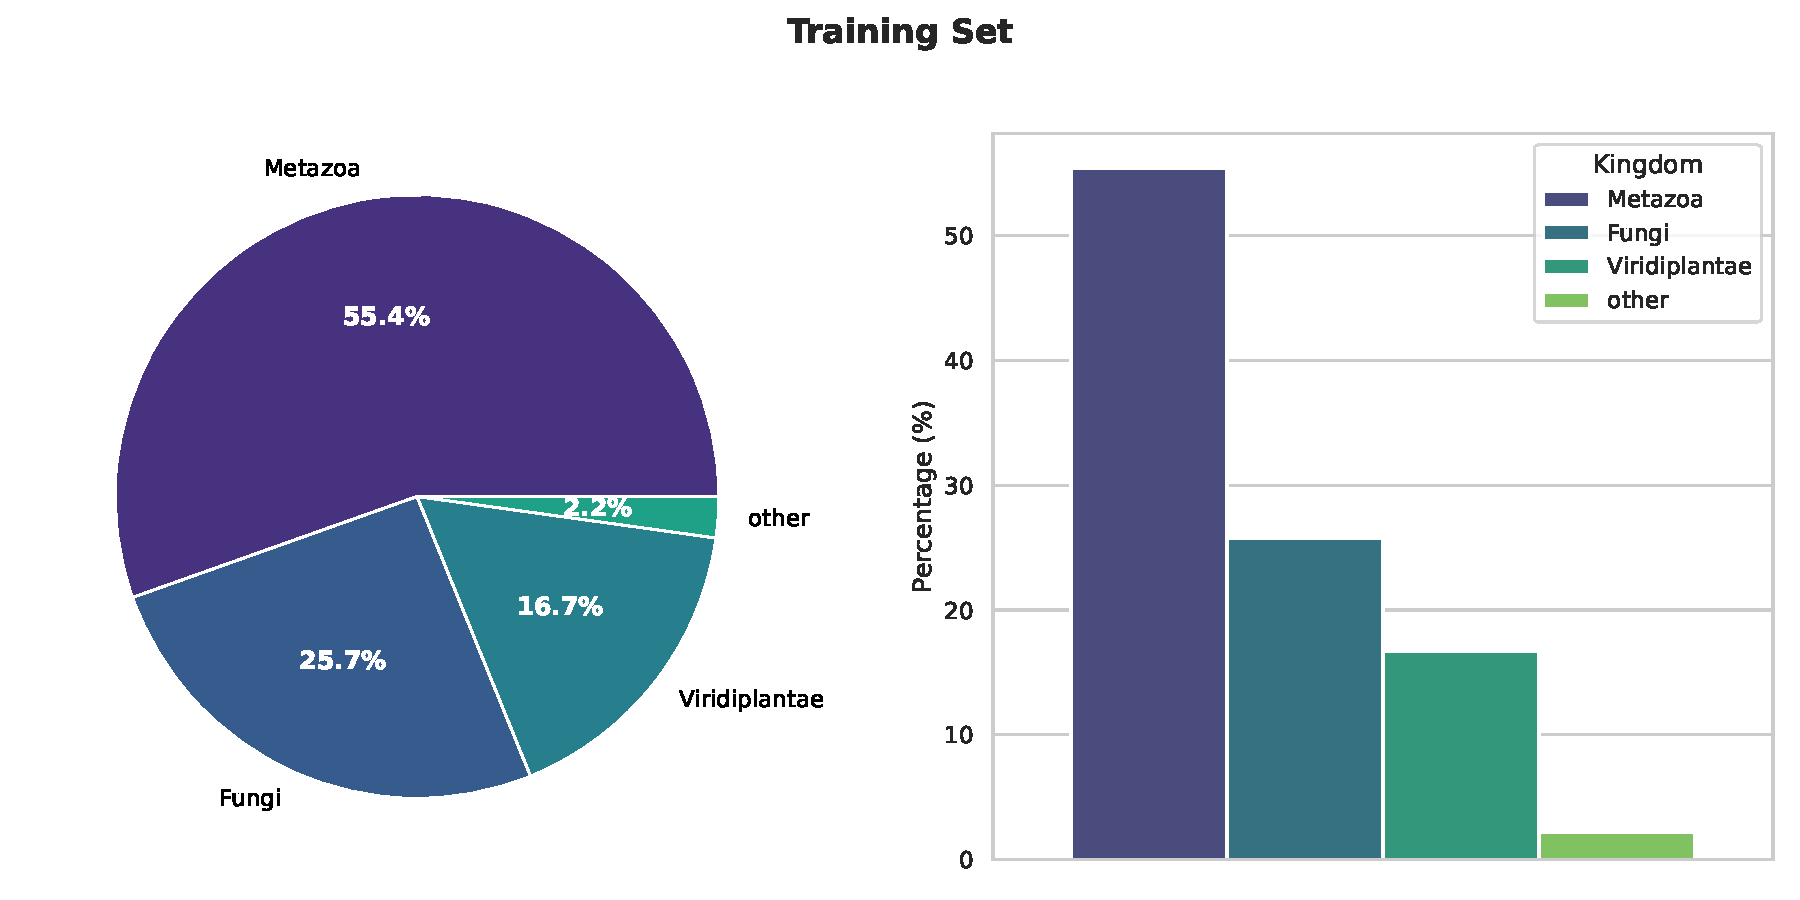
\includegraphics[width=0.49\linewidth]{data/data_analysis/train_kingdoms.pdf}\hfill
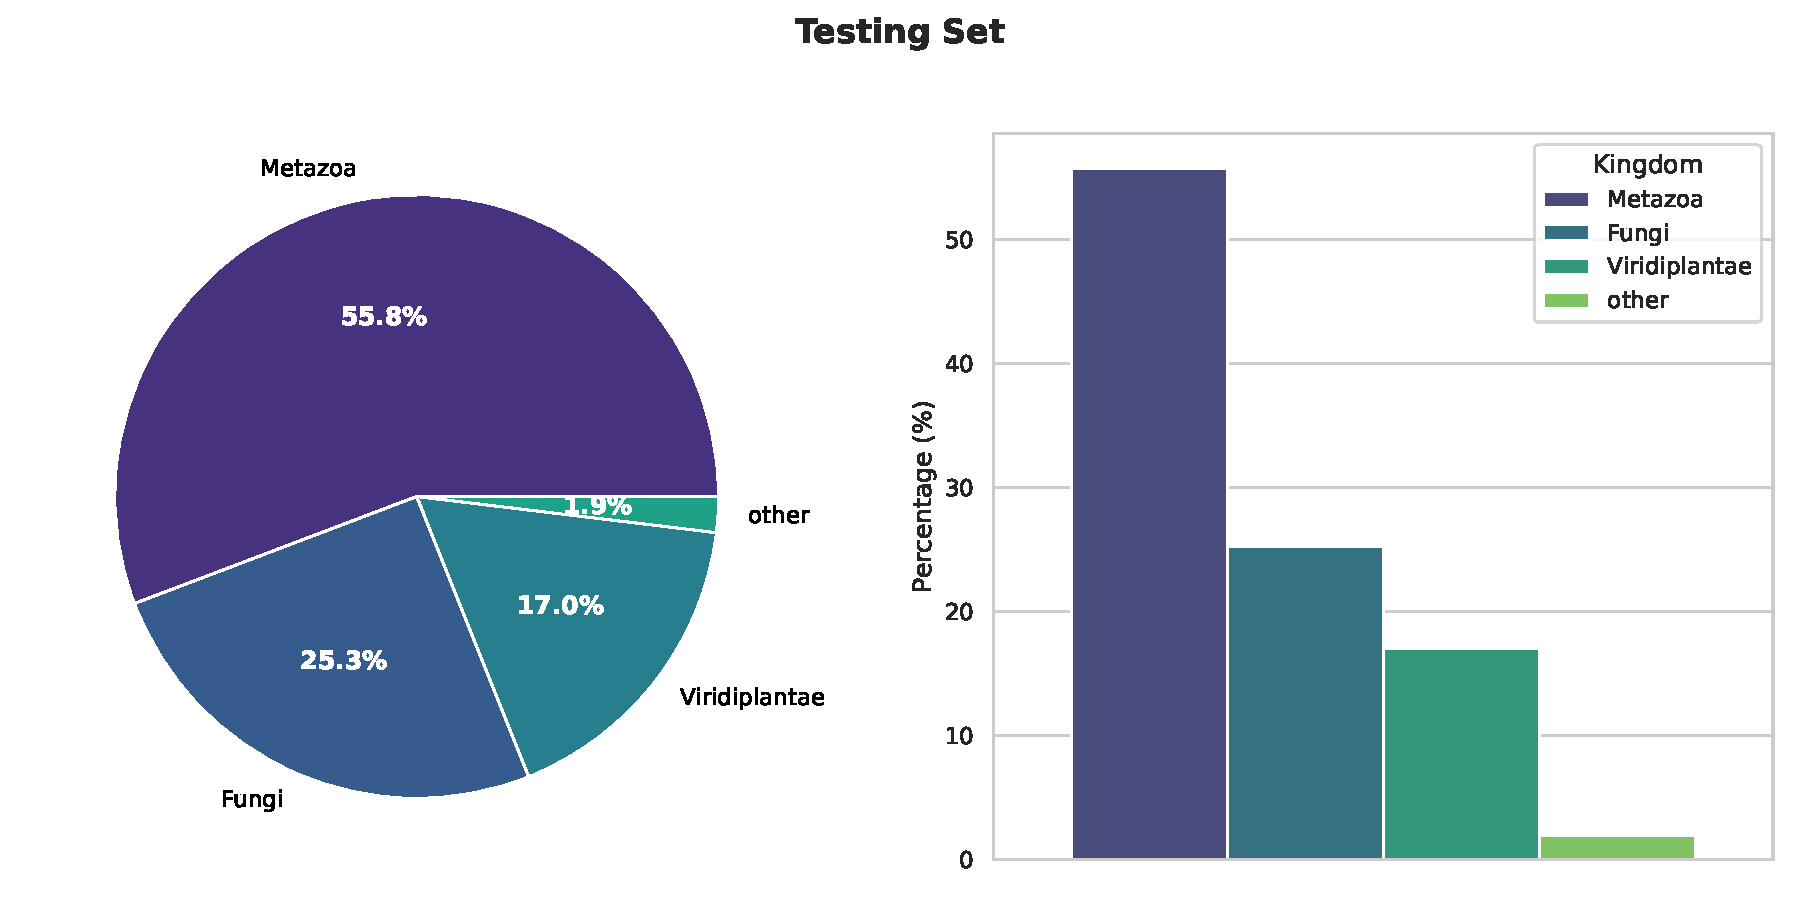
\includegraphics[width=0.49\linewidth]{data/data_analysis/test_kingdoms.pdf}
\caption{Kingdom distribution across the training and benchmarking datasets.}
\label{fig:kingdom}
\end{figure}

\begin{figure}[t]
\centering
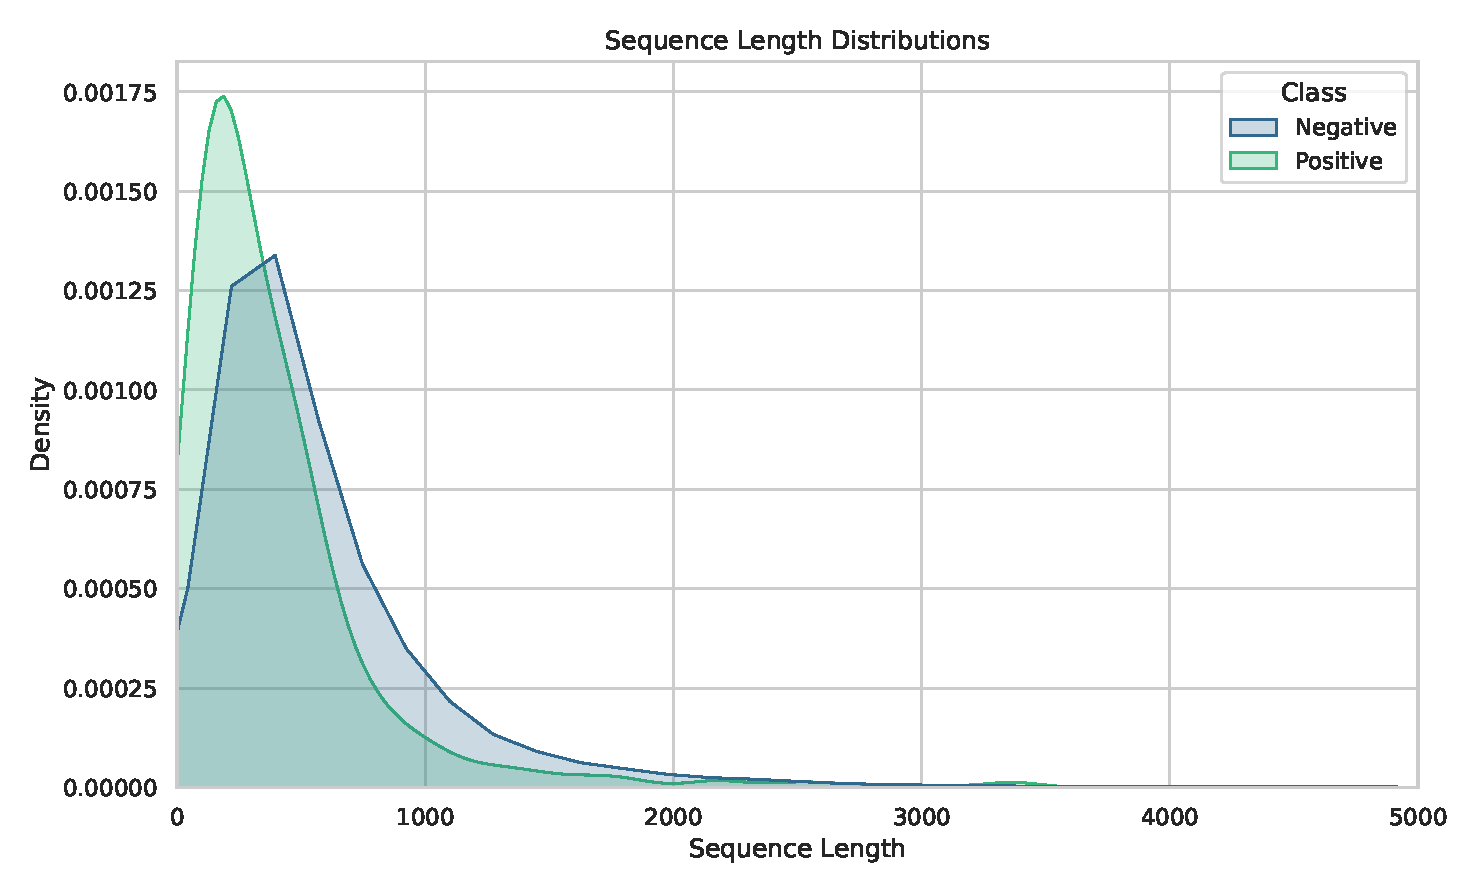
\includegraphics[width=0.49\linewidth]{data/data_analysis/seq_len_dist_by_class.pdf}\hfill
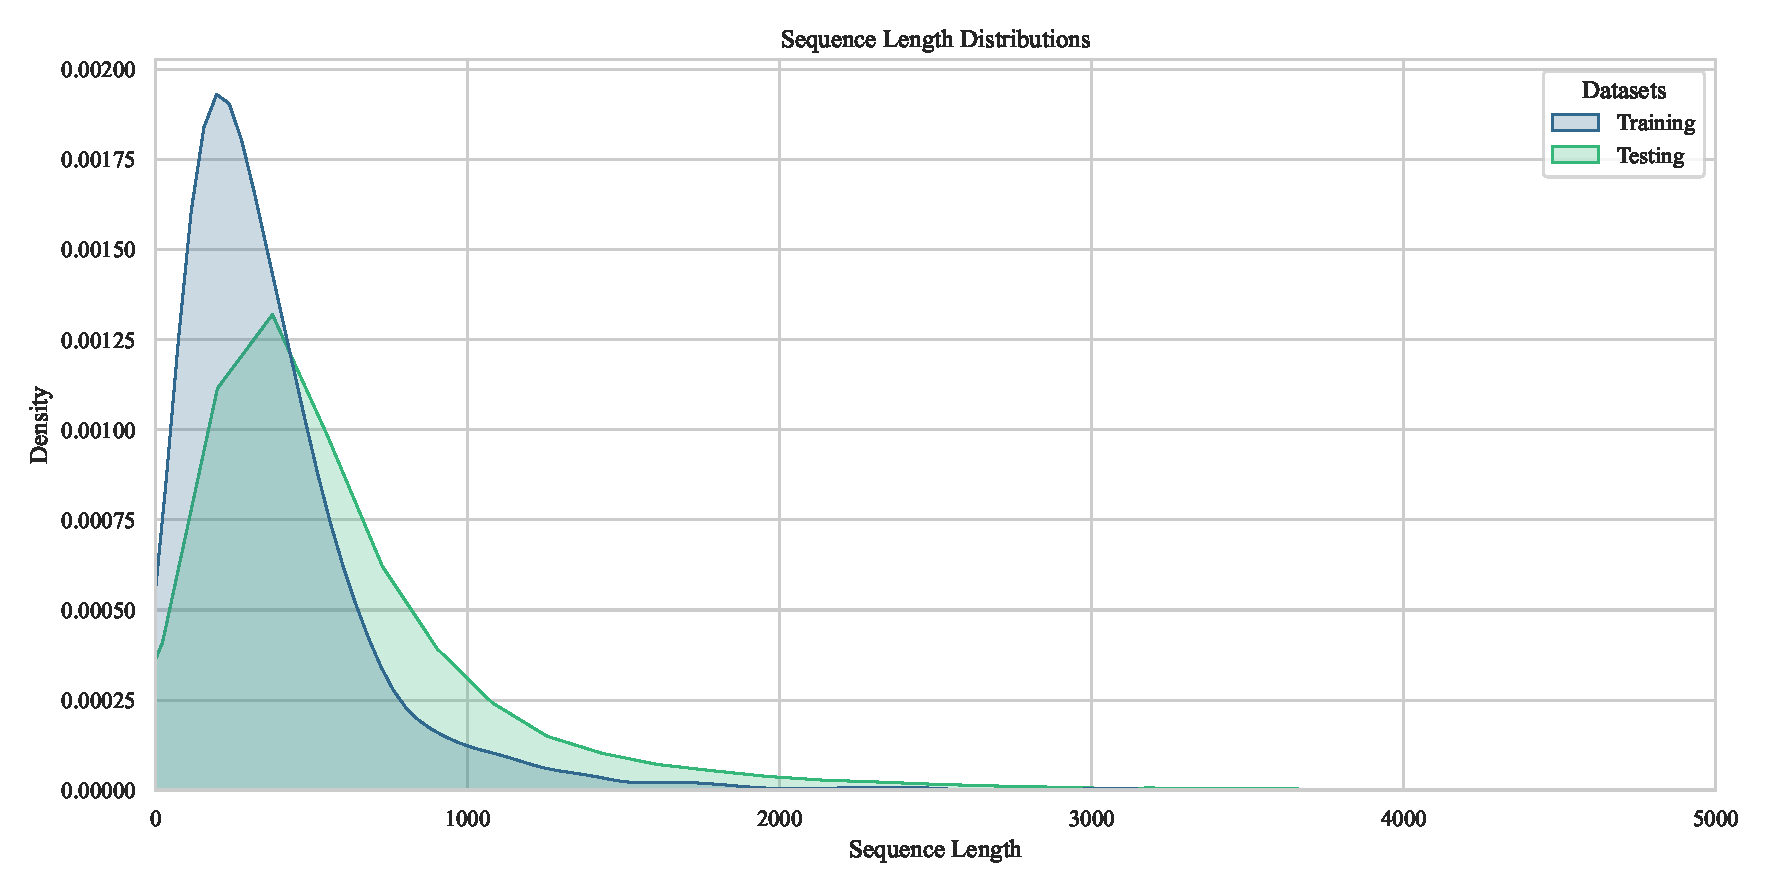
\includegraphics[width=0.49\linewidth]{data/data_analysis/seq_len_dist_by_dataset.pdf}
\caption{Sequence-length distribution: by class and by dataset.}
\label{fig:lendist}
\end{figure}

\begin{figure}[t]
\centering
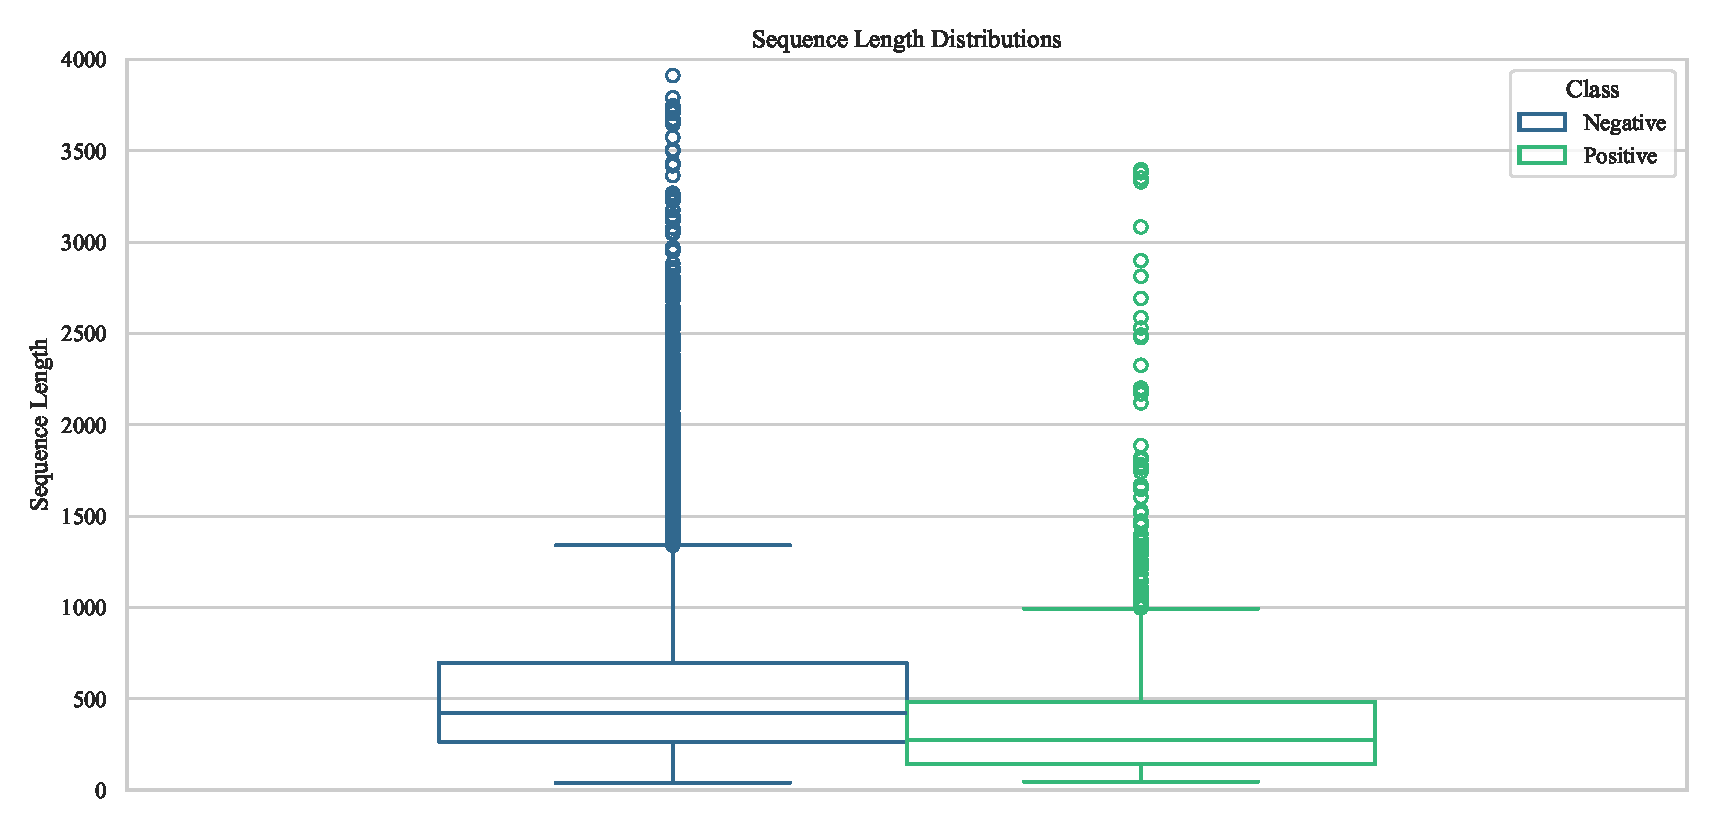
\includegraphics[width=0.49\linewidth]{data/data_analysis/seq_len_boxplot_by_class.pdf}\hfill
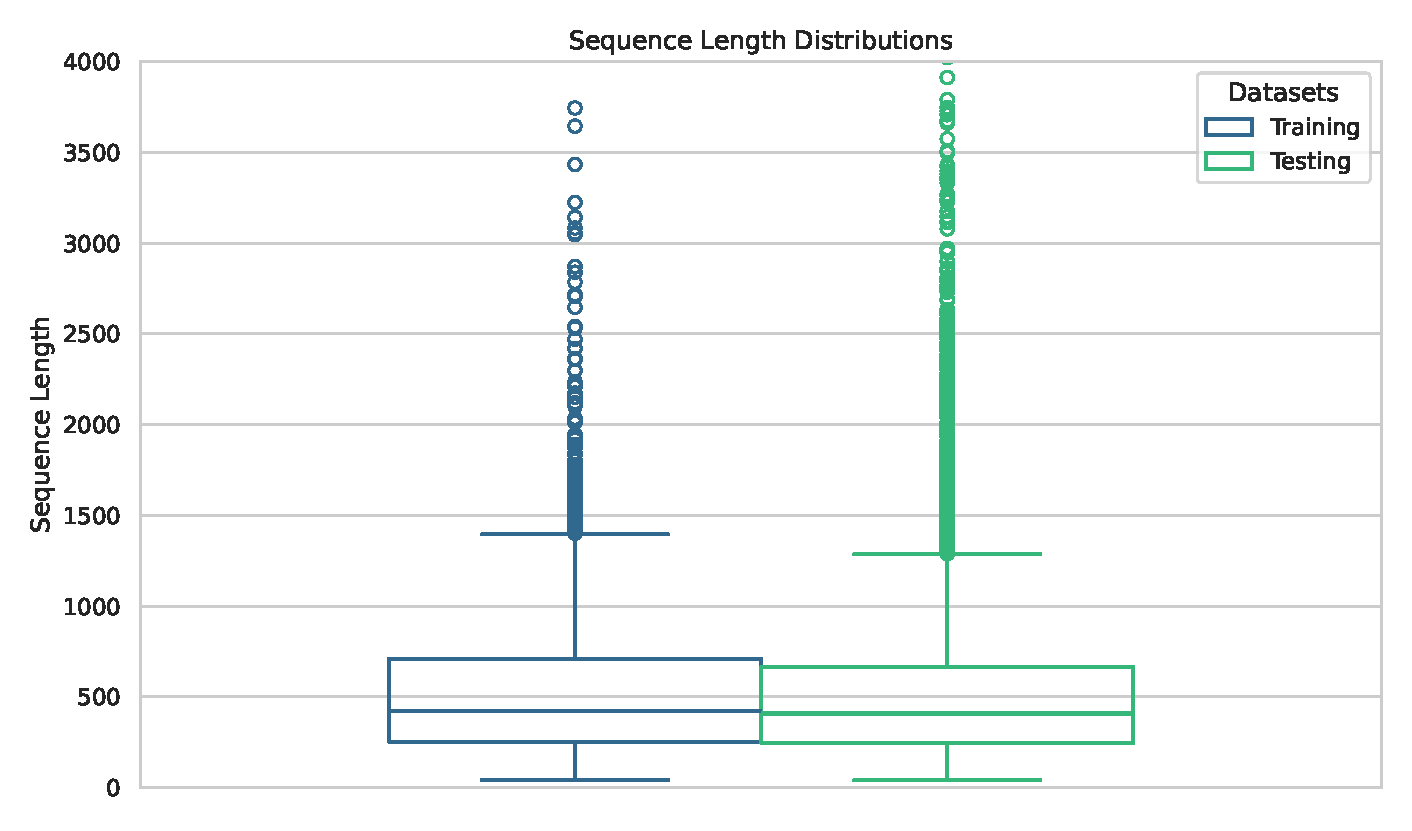
\includegraphics[width=0.49\linewidth]{data/data_analysis/seq_len_boxplot_by_dataset.pdf}
\caption{Sequence-length distribution outliers: by class and by dataset.}
\label{fig:lenout}
\end{figure}

\begin{figure}[t]
\centering
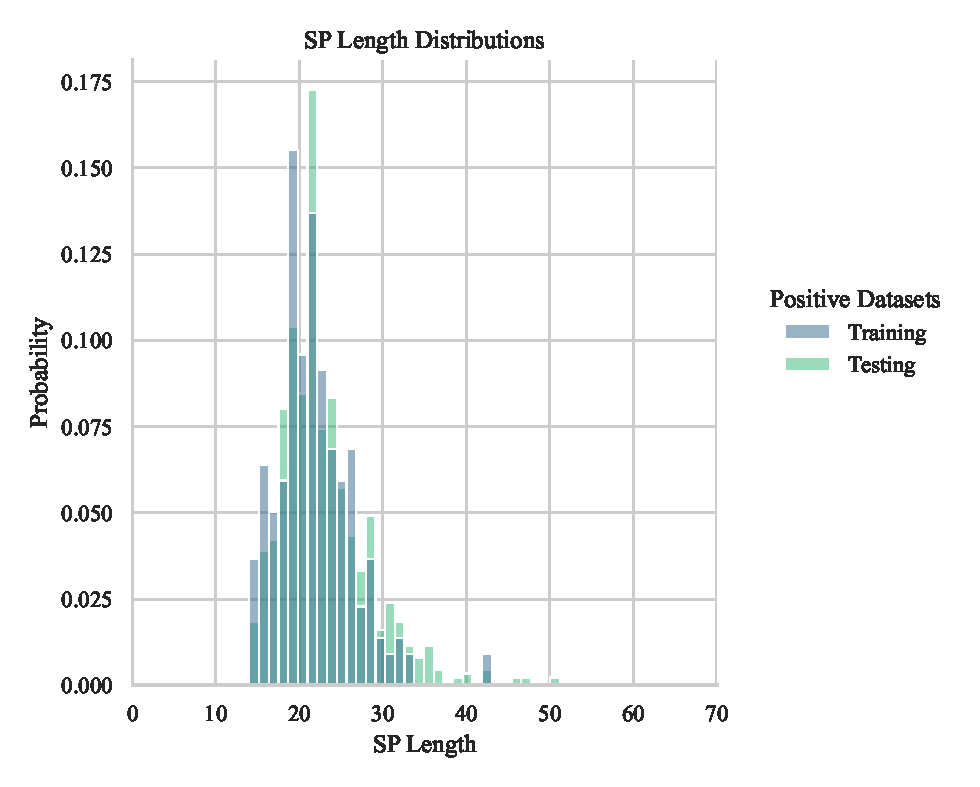
\includegraphics[width=0.7\linewidth]{data/data_analysis/cleavage_len_hist_by_dataset_pos.pdf}
\caption{SP length distribution in the positive datasets.}
\label{fig:splen}
\end{figure}

\subsection{von Heijne}

A custom Python script was used to develop a classical weight-matrix method based on the framework first proposed by von Heijne \cite{ref22} to create a comparative baseline for signal-peptide prediction. This method models the statistical distribution of amino-acid residues within the SP motif using Position-Specific Weight Matrices (PSWMs).

The model was trained on 15-residue sequence motifs extracted from the positive dataset. These motifs were anchored at the cleavage site, spanning 13 residues upstream and 2 residues downstream (positions $-13$ to $+2$), to capture the distinct signatures of the N-, H-, and C-regions. To construct the Position-Specific Probability Matrix (PSPM), residues were processed using a one-hot encoding strategy to count occurrences at each position $j$. To account for sparse data and prevent zero probabilities, pseudocounts were incorporated. The probability $M_{k,j}$ for residue $k$ at position $j$ was calculated as:
\begin{equation}
M_{k,j} = \frac{1 + \sum_{i=1}^{N} \mathbb{I}(s_{i,j}=k)}{N + 20}
\end{equation}
where $N$ is the total number of training sequences, the numerator includes a pseudocount of 1, and the denominator is adjusted by the 20 standard amino acids. To determine the functional significance of each residue, the probability matrix was converted into a log-odds PSWM, normalized against the background distribution $b_k$ derived from the \textit{UniProtKB/Swiss-Prot} amino-acid composition \cite{ref3}:
\begin{equation}
W_{k,j} = \log_2\!\left(\frac{M_{k,j}}{b_k}\right)
\end{equation}
Positive weights indicate residues that are favored or functionally conserved at a given position, while negative values signify selective pressure against them.

To predict the presence of an SP in an uncharacterized query sequence $X$, a sliding-window approach with a fixed length of 15 residues was employed. Given that SPs are localized to the N-terminus, the scan was restricted to the first 90 residues of each sequence. The score for a window was calculated by summing the corresponding weights from the PSWM (Figure~\ref{fig:pswm}):
\begin{equation}
\mathrm{Score}(X \mid W) = \sum_{j=1}^{L} W_{x_j, j}
\end{equation}
The final score for a sequence was the maximum value obtained across all windows within the 90-residue N-terminal segment. This was implemented using \textit{NumPy} for optimized matrix operations. The optimal classification threshold was determined by maximizing the F1 score on the validation data during cross-validation; the PSWM and its threshold were taken jointly from the same best-performing fold.

\begin{figure}[t]
\centering
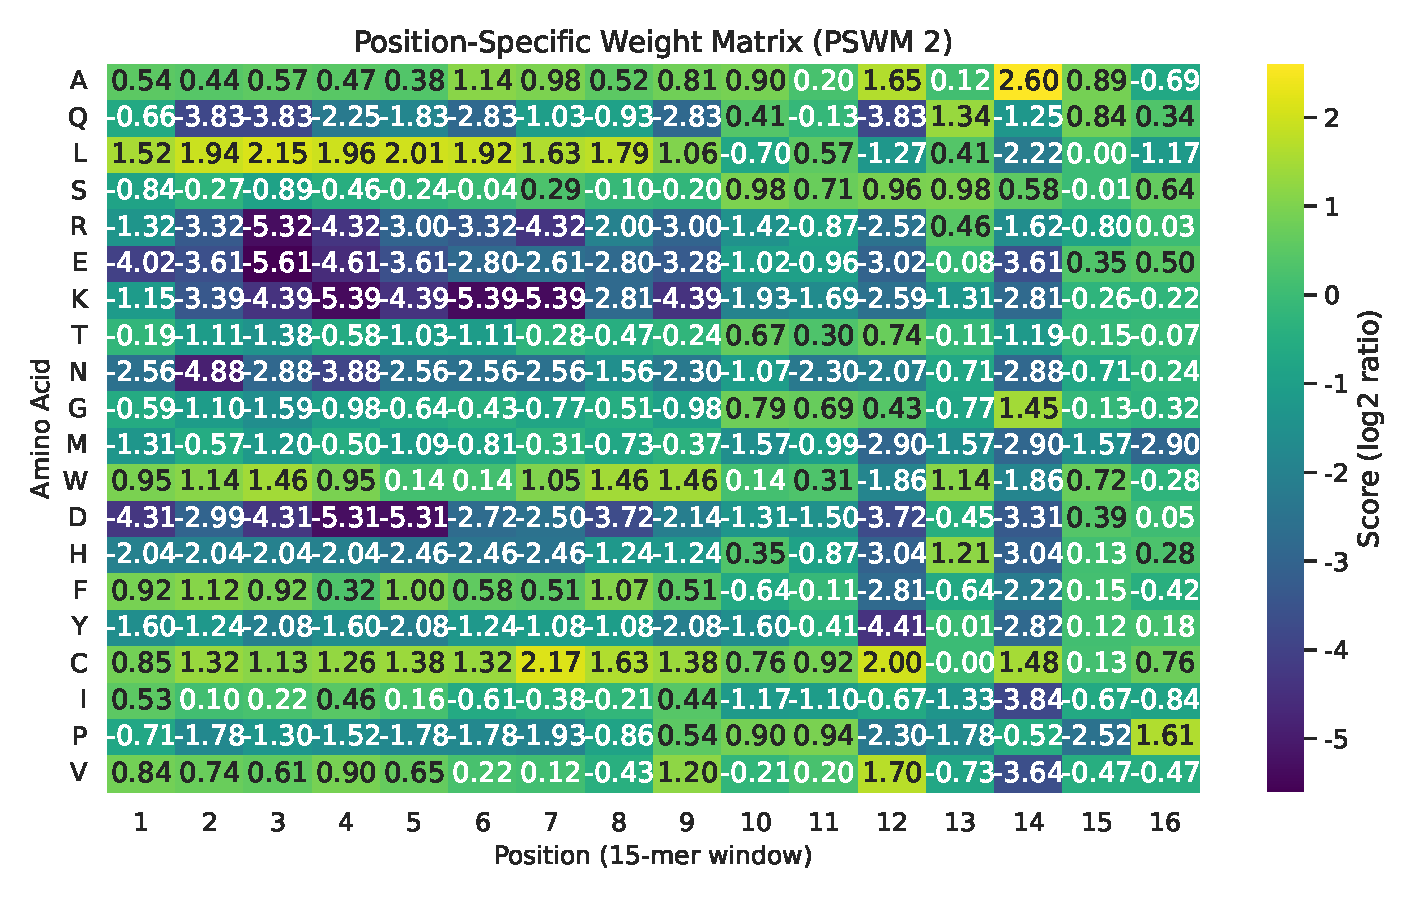
\includegraphics[width=\linewidth]{data/pswm/PSWM_cv_2.pdf}
\caption{The best PSWM derived from the five cross-validation rounds (fold 2).}
\label{fig:pswm}
\end{figure}

\subsection{Support Vector Machine (SVM)}

Support Vector Machines are supervised learning algorithms that use an optimal hyperplane in an $n$-dimensional feature space to categorize data. This hyperplane is defined by the subset of training points that maximize the classification margin, known as support vectors. We used a ``Soft Margin'' formulation to deal with datasets that are not fully linearly separable, including slack variables ($\xi_i$) to accept degree-controlled misclassifications and outliers.

For non-linearly separable tasks, the feature space is mapped into a higher-dimensional space where linear separation becomes feasible. To avoid explicitly defining high-dimensional transformations, we employed the ``kernel trick,'' allowing direct evaluation of inner products in the transformed space via a kernel function $K(x_i, x_j)$. The decision boundary is defined by $\langle w, x\rangle + b = 0$, and the model is trained by solving:
\begin{equation}
\min_{w,b,\xi}\ \left(\tfrac{1}{2}\lVert w\rVert^2 + C\sum_i \xi_i\right)
\quad\text{s.t.}\quad y_i(w^T x_i + b) \geq 1-\xi_i,\ \xi_i \geq 0
\end{equation}
where $C$ is the regularization parameter. The Radial Basis Function (RBF) kernel was selected to capture non-linear relationships between sequence features.

Protein sequences were transformed into 39-dimensional numerical feature vectors. The feature set was divided into two categories:
\begin{enumerate}
\item \textbf{Baseline Compositional Features (n=20):} the global amino-acid composition within the first 40 N-terminal residues, capturing the relative enrichment of residues such as leucine and alanine in the SP hydrophobic core.
\item \textbf{Context-Dependent Physicochemical Features (n=19):} computed with sliding windows over several biological scales:
\begin{itemize}
\item \textit{Hydrophobicity and Aliphaticity (n=6):} window size 6, Kyte--Doolittle scale \cite{ref15}.
\item \textit{Secondary-Structure Propensity (n=6):} $\alpha$-helix and $\beta$-sheet propensities, window size 9, Chou--Fasman scales \cite{ref9,ref10}.
\item \textit{Residue Charge (n=4):} window size 3.
\item \textit{Transmembrane Propensity (n=3):} window size 7, transmembrane-tendency scale \cite{ref24}.
\end{itemize}
\end{enumerate}

The SVM classifier was developed using a five-fold cross-validation procedure. Hyperparameter optimization was performed via a systematic grid search on the training folds over the regularization parameter $C \in \{0.1, 1, 10, 100\}$ and the kernel coefficient $\gamma \in \{\mathrm{scale}, 0.01, 0.1, 1.0\}$, with the Matthews Correlation Coefficient (MCC) on the validation fold as the selection criterion. To refine the feature set, a class-weighted Random Forest (RF) classifier was concurrently employed to compute Gini feature importances; the SVM MCC was then evaluated across progressively larger subsets of the top-ranked features, retaining the subset that maximized validation MCC. A second grid search over the same $C$ and $\gamma$ ranges was finally run on the selected feature subset to fix the final model, which was compared against an all-features baseline.

\subsection{Feed-Forward Neural Network (FFNN)}

As an additional non-linear classifier, a feed-forward neural network was trained on the same 39 biochemical features used by the SVM, enabling a controlled comparison of model families on an identical representation. The features were standardized (fit on the training folds only), and a small architecture search over one and two hidden layers was evaluated by five-fold cross-validation on the same folds, selecting the configuration with the highest mean validation MCC. The selected network has a single hidden layer of 64 ReLU units and was trained with the Adam optimizer (learning rate $10^{-3}$, $L_2$ regularization $\alpha=10^{-3}$, batch size 64, up to 400 epochs).

The strong class imbalance ($\approx 8{:}1$) was handled in two complementary ways: seeded oversampling of the minority class during training, and tuning of the decision threshold for maximum MCC on the pooled out-of-fold predictions, so that the benchmarking set is never used for threshold selection. Training curves for the selected architecture are shown in Figure~\ref{fig:ffnn_curves}.

\subsection{Performance Assessment}

The performance of the binary classifiers was evaluated using a comprehensive suite of quantitative metrics, all derived from the confusion matrix, which cross-references the experimentally verified ground truth against the model's predictions. The $2\times 2$ confusion matrix yields four outcomes: True Positives (TP), True Negatives (TN), False Positives (FP, Type~I error) and False Negatives (FN, Type~II error). To provide a balanced assessment under class imbalance, the following metrics were computed using validated \textit{Scikit-learn} implementations.

The Matthews Correlation Coefficient (MCC) only achieves a high score if the classifier performs well across all four quadrants of the confusion matrix; its values range from $-1$ to $+1$:
\begin{equation}
\mathrm{MCC} = \frac{(TP\cdot TN)-(FP\cdot FN)}{\sqrt{(TP+FP)(TP+FN)(TN+FP)(TN+FN)}}
\end{equation}
Accuracy quantifies the proportion of correct predictions, $\mathrm{ACC}=(TP+TN)/(TP+TN+FP+FN)$; Precision (PPV) $=TP/(TP+FP)$ quantifies the reliability of positive predictions; Recall (TPR) $=TP/(TP+FN)$ measures completeness; and the F1 score is their harmonic mean, $F_1 = 2\,\mathrm{PPV}\cdot\mathrm{TPR}/(\mathrm{PPV}+\mathrm{TPR})$.


\section{Results}

\subsection{Cross-Validation Performance}

The predictive efficacy of the von Heijne and SVM models was first evaluated through five-fold cross-validation. For the vH method, an optimal classification threshold was determined for each fold by maximizing the F1 score on the validation set. The resulting thresholds and F1 scores are summarized in Table~\ref{tab:folds}; the best fold (fold 2) achieved $F_1 = 0.763$ at a threshold of $\mathit{th} = 8.653$, and both the PSWM and threshold of that fold were carried forward to benchmarking. For the SVM model, the cross-validation framework served to identify the optimal feature subset by measuring MCC in each round; the top-20 features of the best round are shown in Figure~\ref{fig:gini}.

\begin{table}[t]
\caption{Per-fold optimal threshold values and F1 scores for the vH method.}
\label{tab:folds}
\centering
\begin{tabular}{lrr}
\toprule
Fold & Optimal Threshold & F1 Score \\
\midrule
1 & 9.226 & 0.728 \\
2 & 8.653 & 0.763 \\
3 & 8.622 & 0.710 \\
4 & 9.563 & 0.705 \\
5 & 9.438 & 0.711 \\
\bottomrule
\end{tabular}
\end{table}

\subsection{Benchmarking on Hold-out Data}

To evaluate final performance, the classifiers were retrained on the complete training set and assessed against the separate benchmarking dataset. The benchmarking results (Table~\ref{tab:benchmark}) confirm the trends observed during cross-validation: both feature-based models substantially outperform the von Heijne baseline, with the SVM achieving the highest MCC (0.839) and the FFNN the highest recall (0.873). The raw classification counts further illustrate the SVM's superior ability to minimize both false positives and false negatives (Figure~\ref{fig:cm}): the von Heijne baseline yields 86 FP and 50 FN, whereas the SVM yields only 25 FP and 37 FN.

\begin{table}[t]
\caption{Benchmarking performance on the hold-out dataset (221 positives, 1816 negatives).}
\label{tab:benchmark}
\centering
\begin{tabular}{lccccc}
\toprule
Model & Acc. & Prec. & Rec. & $F_1$ & MCC \\
\midrule
von Heijne PSWM         & 0.933 & 0.665 & 0.774 & 0.715 & 0.680 \\
SVM (all features)      & 0.971 & 0.889 & 0.833 & 0.860 & 0.844 \\
SVM (selected features) & 0.970 & 0.880 & 0.833 & 0.856 & 0.839 \\
FFNN                    & 0.962 & 0.798 & 0.873 & 0.834 & 0.813 \\
\bottomrule
\end{tabular}
\end{table}

The Gini-importance analysis is biologically coherent: averaged over the five folds, the most important features are \texttt{max\_hydrophobicity} (0.092), \texttt{tm\_position} (0.065), \texttt{max\_aliphacity} (0.061) and \texttt{mean\_hydrophobicity} (0.057), with the ten most important features accounting for roughly 51\% of the total importance and the ranking remaining stable across folds. This matches the biology of the problem, in which the discriminative signal is the hydrophobic h-region of the signal peptide, and explains why charge and secondary-structure descriptors contribute comparatively little.

\begin{figure}[t]
\centering
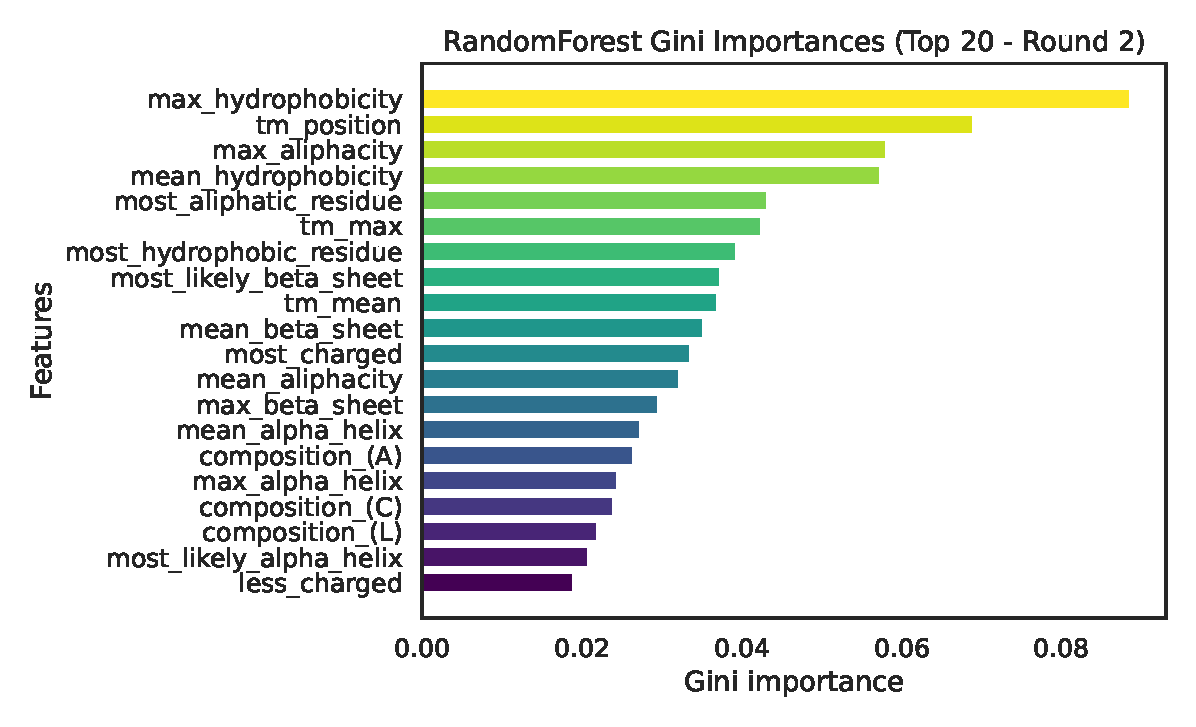
\includegraphics[width=0.85\linewidth]{data/svm/top_20_features_2.pdf}
\caption{Top-20 training features chosen by the cross-validation framework (best round).}
\label{fig:gini}
\end{figure}

\begin{figure}[t]
\centering
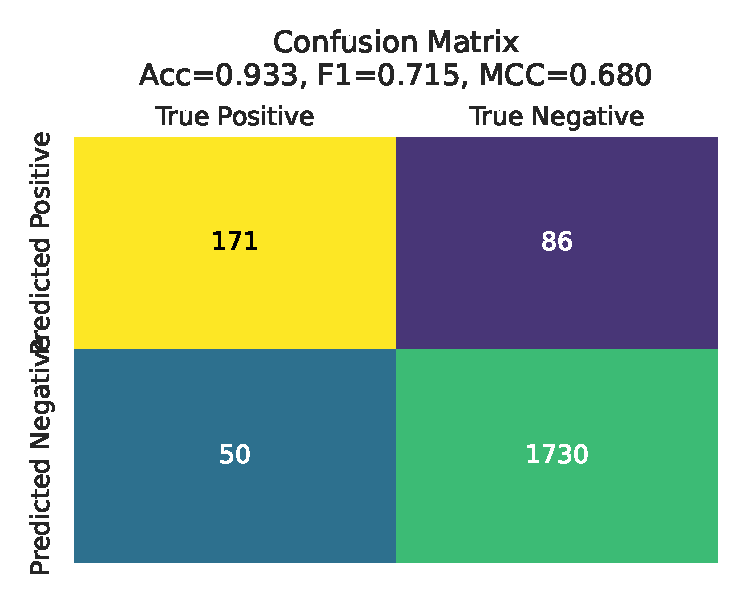
\includegraphics[width=0.49\linewidth]{data/pswm/confusion_matrix.pdf}\hfill

\includegraphics[width=0.49\linewidth]{{data/svm/confusion_matrix_Selected features}.pdf}
\caption{Confusion matrices on the benchmarking set: von Heijne (left) and SVM with selected features (right).}
\label{fig:cm}
\end{figure}

\subsection{Feed-Forward Neural Network}

On the benchmarking set the FFNN reached MCC 0.813 and F1 0.834 (accuracy 0.962, precision 0.798, recall 0.873; Table~\ref{tab:benchmark}), comparable to the SVM and with the highest recall of all models---reflecting the effect of the minority-oversampling and MCC-based threshold tuning. The per-fold training curves of the selected architecture (Figure~\ref{fig:ffnn_curves}) show stable convergence, and the confusion matrix on the benchmarking set is shown in Figure~\ref{fig:ffnn_cm}. The close agreement between the SVM and FFNN, two different model families trained on identical features, indicates that most of the discriminative signal is already captured by the physicochemical feature representation rather than by the choice of classifier.

\begin{figure}[t]
\centering
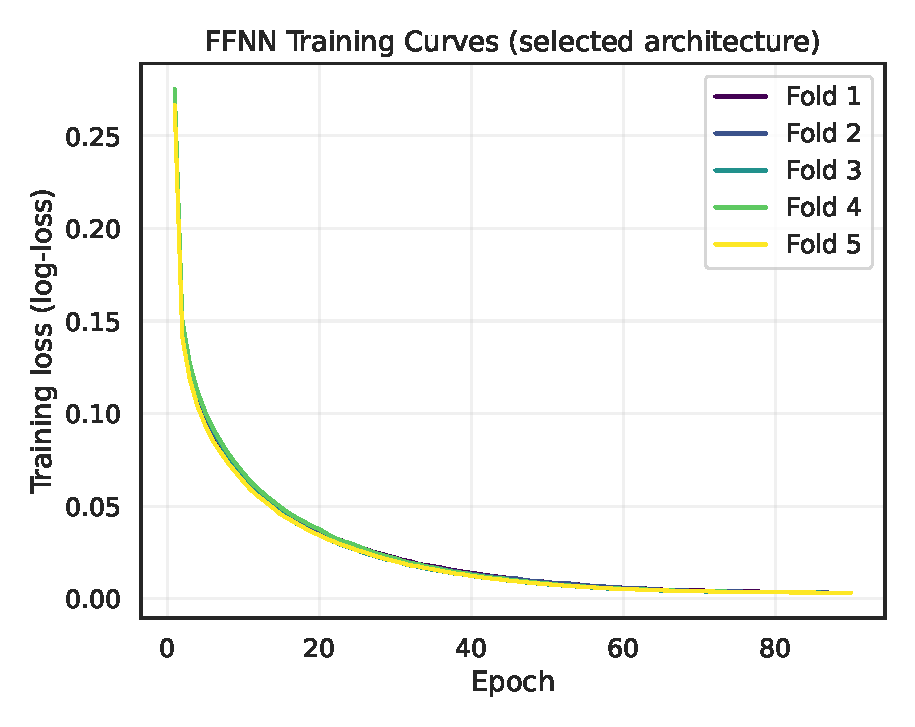
\includegraphics[width=0.75\linewidth]{data/ffnn/training_curves.pdf}
\caption{FFNN training loss per epoch across the five cross-validation folds (selected architecture).}
\label{fig:ffnn_curves}
\end{figure}

\begin{figure}[t]
\centering
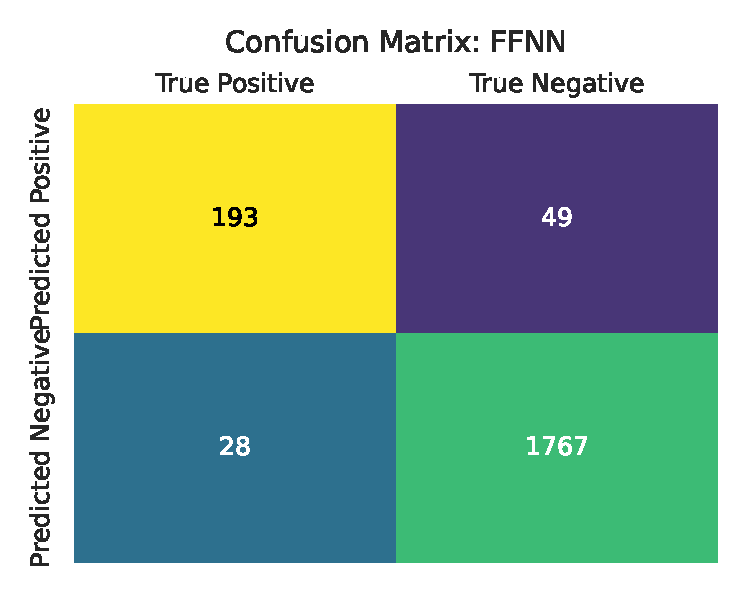
\includegraphics[width=0.5\linewidth]{data/ffnn/confusion_matrix.pdf}
\caption{Confusion matrix of the FFNN on the benchmarking set.}
\label{fig:ffnn_cm}
\end{figure}

\subsection{Analysis of Misclassifications: FP and FN Profiles}

A detailed analysis of misclassified sequences was conducted to identify common sources of error. Transmembrane (TM) proteins make up only 12.1\% of the negative set, yet they are strongly over-represented among the false positives. As shown in Table~\ref{tab:fpr}, the false-positive rate restricted to TM-containing sequences is substantially higher than the overall FPR for both models: the von Heijne method misclassifies 27.2\% of TM negatives (versus an overall FPR of 4.7\%), confirming that a hydrophobic transmembrane helix is readily mistaken for a cleavable h-region by a purely hydrophobicity-based PSWM. The SVM, which receives explicit transmembrane-propensity and positional features, reduces the TM-domain FPR to 6.1\% (overall FPR 1.4\%) and lowers the transmembrane fraction among its false positives from 57\% to 44\%. The biochemical features therefore partially resolve the principal confounder, although the residual enrichment shows that the signal-peptide / transmembrane distinction is not fully solved.

\begin{table}[t]
\caption{Overall vs.\ TM-domain false-positive rate (FPR) on the benchmarking set.}
\label{tab:fpr}
\centering
\begin{tabular}{lrr}
\toprule
Model & Overall FPR & TM-domain FPR \\
\midrule
vH  & 0.047 & 0.272 \\
SVM & 0.014 & 0.061 \\
\bottomrule
\end{tabular}
\end{table}

For the vH method, the sequence logo was computed for all 15-residue fragments of the false negatives in the training dataset and compared to the expected logo (Figure~\ref{fig:logo}). The comparison makes it evident that false negatives may arise from a different composition of the cleavage-site context than expected.

\begin{figure}[t]
\centering
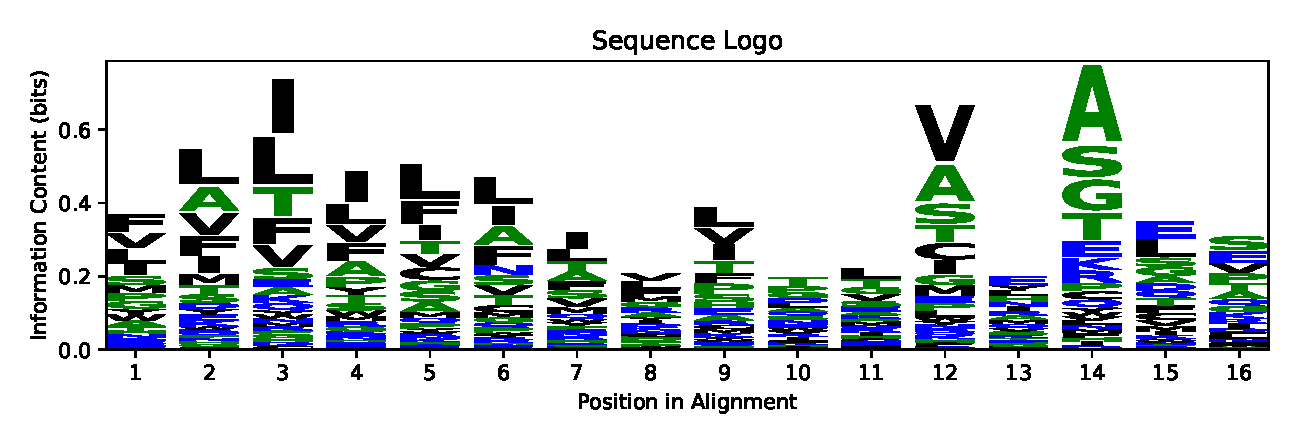
\includegraphics[width=0.49\linewidth]{data/results_analysis/fn_sp_15_sequence_logo.pdf}\hfill
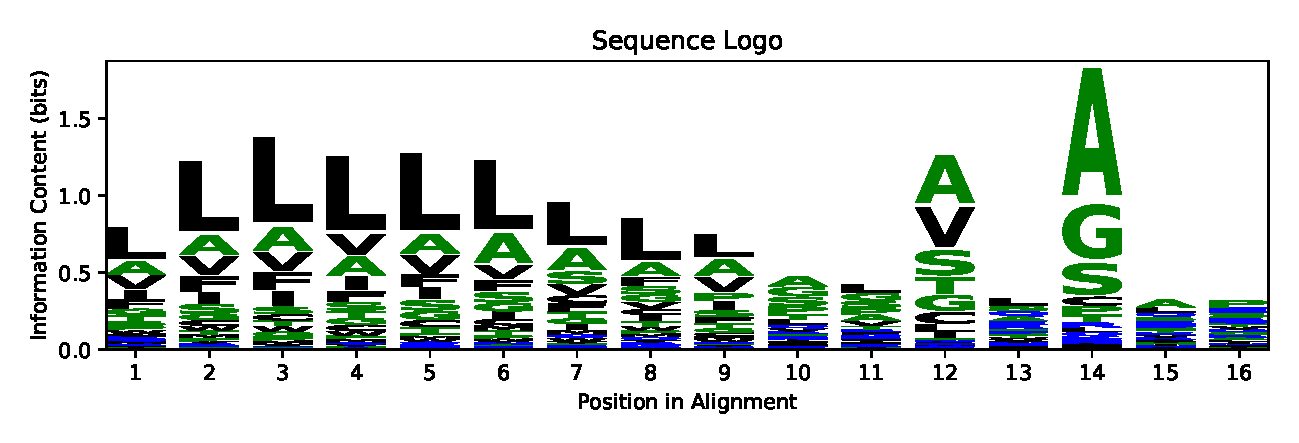
\includegraphics[width=0.49\linewidth]{data/results_analysis/train_sp_15_sequence_logo.pdf}
\caption{Sequence logos: false negatives (left) and expected (right).}
\label{fig:logo}
\end{figure}


\section{Conclusions}

Three computational approaches for the prediction of signal peptides in eukaryotic proteins were systematically evaluated in this work: the traditional von Heijne (vH) positional score matrix, a Support Vector Machine (SVM), and a feed-forward neural network (FFNN). We sought to ensure that our results represent the genuine generalization capacity of the models rather than data artifacts by using a carefully selected dataset of empirically validated secretory and non-secretory proteins, controlled by stringent quality filters and a seeded, homology-aware train--test separation.

Our analysis demonstrates that while the vH method effectively captures conserved sequence motifs adjacent to the cleavage site, its predictive efficacy is constrained by its reliance on local positional statistics and its limited sensitivity to global physicochemical trends. In contrast, the feature-based classifiers---incorporating amino-acid composition, physicochemical properties, structural propensities, and context-dependent windowed features---exhibited significantly superior performance in both cross-validation and independent benchmarking. The SVM and FFNN performed comparably (MCC 0.839 and 0.813), indicating that the physicochemical feature representation, rather than the specific classifier, carries most of the discriminative signal. Feature-importance analysis further substantiated that hydrophobicity patterns, secondary-structure propensities, and transmembrane-tendency scores are critical discriminative features.

The detailed error profiling of all classifiers provided biologically meaningful insights. False positives were predominantly enriched with proteins containing N-terminal transmembrane helices, reflecting the high degree of physicochemical mimicry between these domains and the hydrophobic cores of SPs; quantitatively, the von Heijne TM-domain FPR (0.272) is roughly six times its overall FPR, and the feature-based models substantially attenuate this confounder. Conversely, false negatives were typically associated with atypical SP compositions or non-canonical cleavage-site distributions.

In conclusion, machine-learning models utilizing high-dimensional feature spaces provide the precision and resilience needed for contemporary proteomics, even though traditional motif-based techniques remain useful as transparent, computationally light baselines. Improving SP detection technologies boosts downstream applications in recombinant protein engineering and clinical variant interpretation, promotes large-scale genomics initiatives, and improves the accuracy of functional protein annotation.

\section*{Acknowledgements}
We wish to acknowledge Professors Castrense Savojardo and Matteo Manfredi for their expert advice, insightful feedback, and invaluable guidance throughout the completion of this work.

\section*{Availability}
All code, preprocessing scripts, trained models, and benchmarking datasets used in this study are openly available in the project's GitHub repository: \url{https://github.com/KinitaL/SP_predictors_evaluation}. The repository provides the complete workflow for dataset assembly, feature extraction, von Heijne scoring, SVM and FFNN training, cross-validation, and benchmarking, enabling full reproducibility of the analyses.


\begin{thebibliography}{99}

\bibitem{ref1} B. Alberts et al. \textit{Molecular Biology of the Cell}. W. W. Norton \& Company, 7th edition, 2022.
\bibitem{ref2} J. J. Almagro Armenteros et al. SignalP 5.0 improves signal peptide predictions using deep neural networks. \textit{Nat. Biotechnol.}, 37:420--423, 2019.
\bibitem{ref3} A. Bairoch. Amino-acid composition (\%) in the UniProtKB/Swiss-Prot data bank. \textit{UniProtKB/Swiss-Prot Release Notes}, 2013. Release 2013\_04. Available at: ExPASy ProtScale.
\bibitem{ref4} S. Barash et al. Human secretory signal peptide description by hidden Markov models. \textit{Biochem. Biophys. Res. Commun.}, 294:835--842, 2002.
\bibitem{ref5} D. Brown and S. Breton. Sorting proteins to their target membranes. \textit{Kidney Int.}, 57:816--824, 2000.
\bibitem{ref6} M. Burdukiewicz et al. Prediction of signal peptides in proteins from malaria parasites. \textit{Int. J. Mol. Sci.}, 19:3709, 2018.
\bibitem{ref7} Y. D. Cai, S. L. Lin, and K. C. Chou. Support vector machines for prediction of signal sequences and their cleavage sites. \textit{Peptides}, 24:159--161, 2003.
\bibitem{ref8} J. Chen et al. In silico protein function prediction: the rise of machine-learning-based approaches. \textit{Med. Rev.}, 3:487--510, 2023.
\bibitem{ref9} P. Y. Chou and G. D. Fasman. Conformational parameters for $\alpha$-helix formation. \textit{Adv. Enzymol.}, 47:45--148, 1978.
\bibitem{ref10} P. Y. Chou and G. D. Fasman. Conformational parameters for $\beta$-sheet formation. \textit{Adv. Enzymol.}, 47:45--148, 1978.
\bibitem{ref11} G. E. Crooks, G. Hon, J.-M. Chandonia, and S. E. Brenner. WebLogo: a sequence logo generator. \textit{Genome Res.}, 14:1188--1190, 2004.
\bibitem{ref12} A. Dumitrescu et al. TSignal: A transformer model for signal-peptide prediction. \textit{Bioinformatics}, 39:1347--1356, 2023.
\bibitem{ref13} S. Ghovvati et al. In silico analysis of signal peptides for secretory production of interferon-beta-1b. \textit{Acta Biochim. Pol.}, 65:521--534, 2018.
\bibitem{ref14} K. K. Kandaswamy et al. SPRED: A machine-learning approach for secretory protein identification. \textit{Biochem. Biophys. Res. Commun.}, 391:1306--1311, 2010.
\bibitem{ref15} J. Kyte and R. F. Doolittle. A simple method for displaying the hydropathic character of a protein. \textit{J. Mol. Biol.}, 157:105--132, 1982.
\bibitem{ref16} H. Nielsen et al. A brief history of protein sorting prediction. \textit{Protein J.}, 38:200--216, 2019.
\bibitem{ref17} H. Owji et al. A comprehensive review of signal peptides: structure, roles and applications. \textit{Eur. J. Cell Biol.}, 97:422--441, 2018.
\bibitem{ref18} C. Savojardo et al. DeepSig: deep learning improves signal peptide detection. \textit{Bioinformatics}, 34:1690--1696, 2018.
\bibitem{ref19} M. Steinegger and J. S\"oding. MMseqs2 enables sensitive protein sequence searching for the analysis of massive data sets. \textit{Nat. Biotechnol.}, 35:1026--1028, 2017.
\bibitem{ref20} F. Teufel et al. SignalP 6.0 predicts all five types of signal peptides using protein language models. \textit{Nat. Biotechnol.}, 40:1023--1025, 2022.
\bibitem{ref21} J. P. Vert. Support vector machine prediction of signal peptide cleavage sites. \textit{Pac. Symp. Biocomput.}, 7:649--660, 2002.
\bibitem{ref22} G. von Heijne. A new method for predicting signal sequence cleavage sites. \textit{Nucleic Acids Res.}, 14:4683--4690, 1986.
\bibitem{ref23} S. Zhang et al. Signal peptides: from molecular mechanisms to applications in protein and vaccine engineering. \textit{Biomolecules}, 15:897, 2025.
\bibitem{ref24} G. Zhao and E. London. An amino-acid transmembrane tendency scale. \textit{Protein Sci.}, 15:1987--2001, 2006.

\end{thebibliography}

\end{document}
